\documentclass{article}
\usepackage[margin=1in]{geometry}
\usepackage{amsmath}
\usepackage{amssymb}
\usepackage{algorithm}
\usepackage{graphicx}
\usepackage[noend]{algpseudocode}

\title{CS 6820: Final Project}
\author{Alex Chen, Weiyu Wang, Michael Sosa}
\date{Dec 9, 2017}
\begin{document}
\maketitle

\section{Introduction}

We provide an implementation of Christofides' 3/2-approximation algorithm for the metric traveling salesman problem (TSP) on undirected graphs. In the (symmetric) metric TSP, we are given a complete undirected graph $G$ with vertex set $V = \{v_1, \ldots, v_n\}$ and a cost function $c \colon V \times V \to \mathbb{R} \cup \{\infty\}$ on the edges of $G$ that satisfies the following properties for all vertices $u, v, w \in V$:
\begin{align*}
	c(v, v) &= 0 \\
    c(u, v) &= c(v, u) \\
    c(u, v) + c(v, w) &\geq c(u, w).
\end{align*}
The goal is to output a path $P$ in $G$ that starts at some vertex $v_i$, visits every vertex exactly once, and returns to $v_i$, such that the sum of the costs of every edge in $P$ is minimized.

Christofides' algorithm is as follows:
\begin{enumerate}
	\item Construct a minimum spanning tree $T = (V, E')$ of $G = (V, E)$.
    \item Let $V^-$ be the set of vertices in $T$ with odd degree, and let $K(V^-)$ denote the complete graph of the vertices $V^-$. Compute a minimum-weight perfect matching in $V^-$; this gives an edge set $M$.
    \item Let $G'$ be the multigraph with vertex set $V$ and edge set $E' + M$. Find an Eulerian cycle $C$ in $G'$.
    \item Return the path whose vertices are all of the vertices of $C$ in order, but skipping over duplicates.
\end{enumerate}

Note that in step $2$ of the algorithm, $V^-$ will always have a perfect matching: observe that for the undirected graph $G$, we have that $\sum_{v \in V} d(v)$ is even, as each edge contributes $2$ to the total degree. If we let $V^+$ be the set of even-degree vertices in $G$ and $V^-$ be the set of odd-degree vertices, $\sum_{v \in V^+} d(v)$ is obviously even, so it follows that $\sum_{v \in V^-} d(v)$ is even, and since every vertex in $V^-$ has odd degree, there must be an even number of them. Hence $K(V^-)$ always has a perfect matching.

\section{Implementation}

Our C++ code is broken up into two parts, the first of which contains the implementation of everything other than step $2$, and the second of which contains only step $2$.

For the first part, we encode the graph using an adjacency list representation, where nodes are stored as integers and edges are stored inside structs containing their adjacent nodes and weights. (note that we could even remove the adjacency list were we to assume that the graph must be complete, but because minimum spanning tree and Eulerian cycles exist for non-complete graphs, we chose to generalize).

We use Prim's algorithm to compute the minimum spanning tree. We used a priority queue on the edges and an unordered set (hash set) to store the vertices already in the tree. Because each iteration of Prim's algorithm requires querying and adding to the priority queue, our implementation runs in $O(|E| \log |E|)$ time on a graph $G = (V, E)$. Further optimizations could improve the running time to $O(|E| + |V|\log |V|)$, but this was deemed unimportant as it is not the bottleneck of the algorithm either way.

We use Hierholzer's algorithm to compute an Eulerian cycle on an arbitrary graph where every vertex has even degree. To implement this algorithm we maintain two stacks, a \texttt{forward} stack that stores vertices encountered while exploring the graph, and a \texttt{backward} stack that stores vertices lost when backtracking. On each iteration of the algorithm, we are given a root and travel randomly along edges, deleting them from the graph and adding the vertices to \texttt{forward}, until we return to that root. Since vertices have even degree, we are guaranteed to end at the root. At this point we backtrack along \texttt{forward}, storing the popped nodes in \texttt{backward}, until we come across a node with positive degree. If no such node exists then the algorithm is finished. Otherwise, that node is set as the new root, and the algorithm proceeds. At the end of the algorithm, the nodes in \texttt{forward} are combined with the nodes in \texttt{backward} to form the complete Eulerian cycle. The running time of this algorithm should be $O(|E|)$, since each edge is deleted upon traversal, and retraced at most once while backtracking. However, our running time can only be bounded by $O(|E||V|)$, since we must search the adjacency list of the other node when deleting an edge.

The second part of our code involves step $2$ in Christofides' algorithm: computing a minimum-weight perfect matching in a non-bipartite graph. This part is significantly more involved.

\subsection{Finding a Minimum-Weight Perfect Matching}

The algorithm for finding a minimum-weight perfect matching in a non-bipartite graph combines Edmond's blossom-shrinking algorithm for finding a perfect matching in a non-bipartite graph, and the primal-dual algorithm for finding a minimum-weight perfect matching in a bipartite graph. We give Edmond's LP formulation of a minimum-weight perfect matching on a graph $G = (V, E)$ with variables $x_e$ and costs $c_e$ for each edge $e \in E$:

\begin{alignat*}{3}
	\textrm{minimize}~\sum_{e \in E} c_e x_e&~\textrm{such that}&& \\
	x_e &\in \{0, 1\}  &&\forall e \in E \\
    \sum_{e \in \delta(v)} x_e &= 1 &&\forall v \in V \\
    \sum_{e \in \Delta(S)} x_e &\geq 1 &&\forall S \in \mathcal{O},
\end{alignat*}

where we define 
$$
\delta \colon V \to 2^E~\textrm{by}~\delta(v) = \{e \in E | \textrm{$v$ is an endpoint of $e$}\}
$$ and 
$$
\Delta \colon 2^V \to 2^E~\textrm{by}~\Delta(S) = \{e \in E | \textrm{$e$ has exactly one endpoint in $S$}\},
$$
and $\mathcal{O} = \{S \in 2^V | |S|~\textrm{is odd and}~ |S| \geq 3\}$.

This gives the following dual program, where the dual variables $y_s$ are over $V \cup \mathcal{O}$:
\begin{alignat*}{3}
	\textrm{maximize}~\sum_{v \in V} y_v + \sum_{S \in \mathcal{O}} y_S&~\textrm{such that} && \\
    y_u + y_v + \sum_{e \in \Delta(S)} y_S &\leq c_e &&\forall e=(u, v) \in E \\
    y_S &\geq 0 &&\forall S \in \mathcal{O}.
\end{alignat*}
The modified blossom-shrinking algorithm follows the primal-dual algorithm for weighted bipartite perfect matching: we will store dual values on the nodes and on relevant odd-sets of nodes, and we will store the weights of edges along with their slack, defined as $sl(e) = c_e - y_u - y_v - \sum_{e \in \Delta(S)} y_S$ for all $e = (u, v) \in E$.  At each step of the algorithm, we pick a root vertex $r$, which is unmatched (if every vertex is matched the the algorithm terminates). From $r$ we will use BFS to grow an alternating tree $T$ composed only of edges $e$ with $sl(e) = 0$, i.e. tight edges. Edges that are an even distance (even vertices) from the root inside $T$ are labeled with a +, while edges that are an odd distance (odd vertices) from the root inside $T$ are labeled with a - ; edges outside of $T$ (outside vertices) are labeled with $0$.

While we are growing $T$, we must keep track of a number of variables to ensure that our dual-changing phase does not break any constraints. In particular, we must keep track of the slacks of all non-tight edges connecting an even vertex to an outside vertex, half the slacks of all non-tight edges connecting an even vertex to another even vertex (since the slacks on these vertices will decrease by twice the dual change), and the duals of all odd blossoms inside $T$ (we shall refer to a set in $\mathcal{O}$ as a blossom; an odd blossom is just a blossom with a - label). We will continue growing $T$ until one of three things happens:

\begin{itemize}
	\item We come across a tight edge that connects two even vertices in $T$. In this case have found a blossom; we shrink it into a node. We find the blossom by simultaneously following the parent pointers of both nodes until we reach the least common ancestor.
 	\item We come across a tight edge that connects an even vertex in $T$ to an unmatched outside vertex. In this case we have found an augmenting path; convert this into an augmenting path in the original graph (without blossoms) and take the symmetric difference with the original matching. Then we repeat the process with another unmatched node.
    \item We get stuck, i.e. the tree can no longer be grown. In this case, we take the tightest non-tight constraint, that is, the edge $e$ or set $S$ for which $sl(e)$ is smallest if $e$ is an even-outside edge, $sl(e)/2$ is smallest if $e$ is an even-even edge, or $y_S$ if $S$ is a blossom. Call this value $m$. The duals are are modified by adding $m$ to all even vertices and subtracting $m$ from all odd vertices (note that the duals on individual vertices can be negative). This will either make an edge tight, in which case we continue with the BFS on $T$, or it will make the dual of a blossom $0$. In the latter case, we can expand the blossom back into its constituent nodes, and continue trying to expand $T$.
\end{itemize}

% We provide the following pseudocode for the above procedure:

% \begin{algorithm}
% \caption{Finding an Augmenting Path}
% \begin{algorithmic}[1]
% \Function{find\_augmenting\_path:}{}
% \If {every vertex is matched} \Return 
% \EndIf
% \State Pick an unmatched vertex $v$ and label it $+$
% \State Initialize priority queues $q_{+, 0}$, $q_{+, +}$, and $q_\mathcal{O}$
% \State Initialize a queue $bfs$ and push $v$ onto $bfs$
% \While {$bfs$ is not empty} 
% \State Pop $u$ from $bfs$
% \For {each neighbor $u'$ of $u$}
% \EndFor
% \EndWhile
% \EndFunction
% \end{algorithmic}
% \end{algorithm}

On each iteration of the \texttt{find\_augmenting\_path} subprocedure, we initialize three priority queues, which we will label $q_{+, +}$ for the slacks of even-even edges, $q_{+, 0}$ for the slacks of even-outside edges, and $q_{\mathcal{O}}$ for the duals on blossoms. Whenever we encounter an appropriate edge, we will insert it into the corresponding priority queue. Then, once the BFS is stuck, we will extract the minimum value from each of the queues, take the minimum among those, and update the duals accordingly. 

In order to avoid having to update the duals and edge slacks many times throughout a single iteration of the \texttt{find\_augmenting\_path} procedure, we utilize the idea that the tree only expands. Namely, we will consider each update to the duals as an \textit{update step}. Suppose that there are $n$ update steps. Observe that for each vertex $v$, there is some starting update step $k$ from which all of the updates $k, k+ 1, \ldots n$ are applied. If we store the cumulative sum of update amounts $\epsilon_i$ from $1$ to $k$ for each number $k$ into an array $C$, then the duals on each vertex $v$ can be computed by storing the first update time $t_v$: if $x_v$ is the original dual value on $v$ and $y_v$ is the actual dual, we have $y_v = x_v + C_n - C_{t_v - 1}$. The only exception  $v$ is consumed by a blossom. In this case we must update the dual values stored on the nodes inside the blossom before removing them from the graph.

The other issue is that the values stored in the priority queues become outdated as the true slacks on the edges decrease. In order to remedy this, we assert that $q_{+, +}$ will store $sl(e) + 2 C_k$ where $k$ is the current update stage, $q_{+, 0}$ will store $sl(e) + C_k$, and $q_\mathcal{O}$ will store $y_S + C_k$. 

\section{Evaluation}

\textbf{Unfortunately, we were unable to get our implementation of the blossom algorithm to work, so we have used a library implementation in conducting these tests.}

\subsection{Runtime}

Because our implementation did not work properly for large test cases, we ended up using a library implementation to compute the minimum cost perfect matching, and combined it with our implementations of the other steps of the algorithm. The library boasts an $O(n^3)$ implementation of the blossom algorithm, and it is certainly the bottleneck, so we expect the total runtime to be $O(n^3)$. Still, it is worthwhile to test the performance of the system empirically. For all of our tests, we will assume that the data lies in $\mathbb{R}^2$ (this was a limitation of the exact TSP solver that we used). We provide the running times of the algorithm, in milliseconds, for a number of nodes from $10$ to $300$. Ideally we'd do further tests with more nodes, but requiring the adjacency list representation of a complete graph meant that we'd need to store $O(n^2)$ edges, so we stopped at $300$ nodes. 

\begin{center}
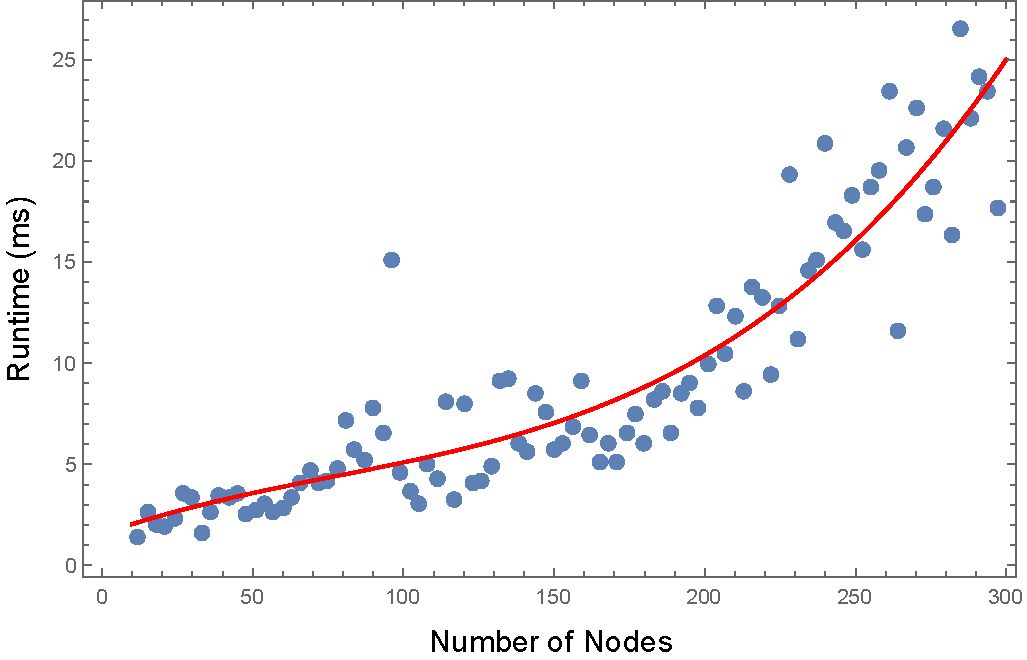
\includegraphics[scale=0.8]{runtime.pdf}
\end{center}

The red line is a cubic fit of the runtime data. Even for $300$ nodes, it took several seconds to construct the edge set of the complete graph from a list of points in the plane. Since even then the algorithm only took $20$ or so milliseconds to run, we can conclude that Christofides' algorithm can be quite fast in practice, especially considering that it needs the adjacency list representation of a potentially very large complete graph.

\subsection{Accuracy}

The main evaluation metric that we wanted to evaluate was the accuracy of Christofides' algorithm in practice. While the cost that Christofides' algorithm outputs can never exceed $3/2$ the actual TSP cost, we consider here its performance on what we consider ``average'' test cases. Our ``average'' test cases consisted of three sets of tests: 
\begin{itemize}
	\item The first set of tests contains points uniformly distributed in a rectangle $[0, M] \times [0, M]$ for some upper bound $M$.
	\item The second set of tests contains points that are concentrated near the origin. In particular, we use a Gaussian distribution on both the $x$ and $y$ coordinates, each of which are centered at $0$.
	\item The third set of tests contains points that are heavily concentrated around a random set of $10$ ``hubs,'' perhaps simulating a ``real-world example'' where points of interest are heavily concentrated near cities and sparsely located elsewhere. 
\end{itemize}

Our goal was to compute the average approximation factor in each of these test scenarios and evaluate whether they differed significantly or at all. In order to do this, we ran each test file on both an exact TSP solver and our implementation of Christofides' algorithm (but using a library implementation of the blossom algorithm). The results are summarized in the graphs below.

\begin{center}
\includegraphics[scale=0.8]{uniform.pdf}
\includegraphics[scale=0.8]{ctc.pdf}
\includegraphics[scale=0.8]{cth.pdf}
\end{center}

The approximation ratio averaged $1.107$, $1.097$, and $1.089$ for the uniform, near-origin, and near-hubs cases, respectively. Given the relatively small number of tests that we performed, the differences between the means are not significant enough to draw any sort of conclusion of whether the distribution of points in the plane affects the expected approximation ratio. 

However, given the distributions of the approximation factors, we can conclude with some confidence that unless an adversarial agent is constructing the graphs, it is unlikely that the average-case performance of Christofides' algorithm will approach its worst-case performance. In combination with its relatively fast runtime -- on some inputs our exact TSP solver took several seconds to compute the answer for a $100$-node test case -- makes it a viable choice for approximating TSP solutions when a polynomial-time algorithm is needed or desired. 

\newpage

\noindent References: 
 
\noindent [1] \textit{Computing Minimum-Weight Perfect Matchings}, William Cook and Andr\'e Rohe \\
{[2]} \textit{Blossom V: a new implementation of a minimum cost perfect matching algorithm}, Vladimir Kolmogorov


\end{document}
